\documentclass{standalone}
\usepackage{tikz}
\usetikzlibrary{patterns, positioning}


\begin{document}
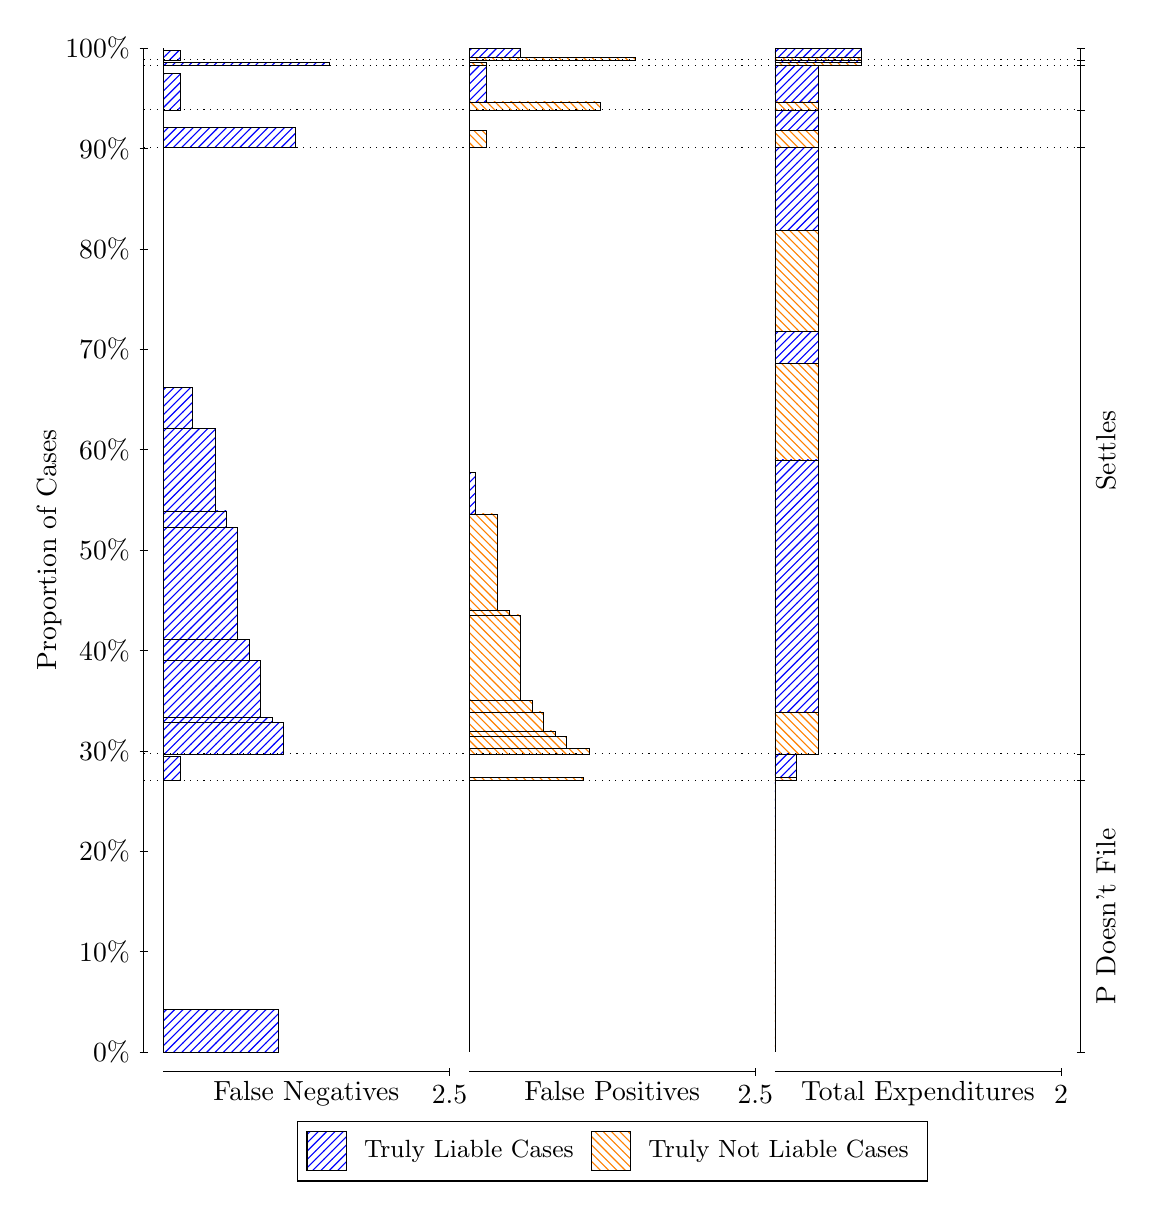
\begin{tikzpicture}
\draw[black, very thin] (1.5,1.75) -- (1.5,14.5);
\node[rotate=90, text=black, anchor=center] at (0.3, 8.125) {Proportion of Cases};
\draw[black, very thin] (1.45,1.75) -- (1.55,1.75);
\node[text=black, anchor=east] at (1.45, 1.75) {0\%};
\draw[black, very thin] (1.45,3.025) -- (1.55,3.025);
\node[text=black, anchor=east] at (1.45, 3.025) {10\%};
\draw[black, very thin] (1.45,4.3) -- (1.55,4.3);
\node[text=black, anchor=east] at (1.45, 4.3) {20\%};
\draw[black, very thin] (1.45,5.575) -- (1.55,5.575);
\node[text=black, anchor=east] at (1.45, 5.575) {30\%};
\draw[black, very thin] (1.45,6.85) -- (1.55,6.85);
\node[text=black, anchor=east] at (1.45, 6.85) {40\%};
\draw[black, very thin] (1.45,8.125) -- (1.55,8.125);
\node[text=black, anchor=east] at (1.45, 8.125) {50\%};
\draw[black, very thin] (1.45,9.4) -- (1.55,9.4);
\node[text=black, anchor=east] at (1.45, 9.4) {60\%};
\draw[black, very thin] (1.45,10.675) -- (1.55,10.675);
\node[text=black, anchor=east] at (1.45, 10.675) {70\%};
\draw[black, very thin] (1.45,11.95) -- (1.55,11.95);
\node[text=black, anchor=east] at (1.45, 11.95) {80\%};
\draw[black, very thin] (1.45,13.225) -- (1.55,13.225);
\node[text=black, anchor=east] at (1.45, 13.225) {90\%};
\draw[black, very thin] (1.45,14.5) -- (1.55,14.5);
\node[text=black, anchor=east] at (1.45, 14.5) {100\%};

\draw[black, very thin] (13.4,1.75) -- (13.4,14.5);
\draw[black, very thin] (13.35,1.75) -- (13.45,1.75);
\node[anchor=west] at (13.35, 1.75) {};
\draw[black, very thin] (13.35,5.198) -- (13.45,5.198);
\node[anchor=west] at (13.35, 5.198) {};
\draw[black, very thin] (13.35,5.5369) -- (13.45,5.5369);
\node[anchor=west] at (13.35, 5.5369) {};
\draw[black, very thin] (13.35,13.239) -- (13.45,13.239);
\node[anchor=west] at (13.35, 13.239) {};
\draw[black, very thin] (13.35,13.714) -- (13.45,13.714);
\node[anchor=west] at (13.35, 13.714) {};
\draw[black, very thin] (13.35,14.283) -- (13.45,14.283);
\node[anchor=west] at (13.35, 14.283) {};
\draw[black, very thin] (13.35,14.35) -- (13.45,14.35);
\node[anchor=west] at (13.35, 14.35) {};
\draw[black, very thin] (13.35,14.5) -- (13.45,14.5);
\node[anchor=west] at (13.35, 14.5) {};

\draw[black, very thin, pattern color=blue, pattern=north east lines] (1.75,1.75) rectangle (3.2033,2.2903);
\draw[black, very thin, pattern color=orange, pattern=north west lines] (1.75,2.2903) rectangle (1.75,5.198);
\draw[black, very thin, pattern color=blue, pattern=north east lines] (1.75,5.198) rectangle (1.968,5.5013);
\draw[black, very thin, pattern color=orange, pattern=north west lines] (1.75,5.5013) rectangle (1.75,5.5369);
\draw[black, very thin, pattern color=blue, pattern=north east lines] (1.75,5.5369) rectangle (3.276,5.9381);
\draw[black, very thin, pattern color=blue, pattern=north east lines] (1.75,5.9381) rectangle (3.1307,5.9952);
\draw[black, very thin, pattern color=blue, pattern=north east lines] (1.75,5.9952) rectangle (2.9853,6.7219);
\draw[black, very thin, pattern color=blue, pattern=north east lines] (1.75,6.7219) rectangle (2.84,6.9935);
\draw[black, very thin, pattern color=blue, pattern=north east lines] (1.75,6.9935) rectangle (2.6947,8.4125);
\draw[black, very thin, pattern color=blue, pattern=north east lines] (1.75,8.4125) rectangle (2.5493,8.622);
\draw[black, very thin, pattern color=blue, pattern=north east lines] (1.75,8.622) rectangle (2.404,9.668);
\draw[black, very thin, pattern color=blue, pattern=north east lines] (1.75,9.668) rectangle (2.1133,10.194);
\draw[black, very thin, pattern color=orange, pattern=north west lines] (1.75,10.194) rectangle (1.75,13.239);
\draw[black, very thin, pattern color=blue, pattern=north east lines] (1.75,13.239) rectangle (3.4213,13.497);
\draw[black, very thin, pattern color=orange, pattern=north west lines] (1.75,13.497) rectangle (1.75,13.714);
\draw[black, very thin, pattern color=blue, pattern=north east lines] (1.75,13.714) rectangle (1.968,14.181);
\draw[black, very thin, pattern color=orange, pattern=north west lines] (1.75,14.181) rectangle (1.75,14.283);
\draw[black, very thin, pattern color=blue, pattern=north east lines] (1.75,14.283) rectangle (3.8573,14.314);
\draw[black, very thin, pattern color=orange, pattern=north west lines] (1.75,14.314) rectangle (1.75,14.35);
\draw[black, very thin, pattern color=blue, pattern=north east lines] (1.75,14.35) rectangle (1.968,14.469);
\draw[black, very thin, pattern color=orange, pattern=north west lines] (1.75,14.469) rectangle (1.75,14.5);
\draw[black, very thin, pattern color=orange, pattern=north west lines] (5.6333,1.75) rectangle (5.6333,4.6577);
\draw[black, very thin, pattern color=blue, pattern=north east lines] (5.6333,4.6577) rectangle (5.6333,5.198);
\draw[black, very thin, pattern color=orange, pattern=north west lines] (5.6333,5.198) rectangle (7.0867,5.2337);
\draw[black, very thin, pattern color=blue, pattern=north east lines] (5.6333,5.2337) rectangle (5.6333,5.5369);
\draw[black, very thin, pattern color=orange, pattern=north west lines] (5.6333,5.5369) rectangle (7.1593,5.6023);
\draw[black, very thin, pattern color=orange, pattern=north west lines] (5.6333,5.6023) rectangle (6.8687,5.7532);
\draw[black, very thin, pattern color=orange, pattern=north west lines] (5.6333,5.7532) rectangle (6.7233,5.8281);
\draw[black, very thin, pattern color=orange, pattern=north west lines] (5.6333,5.8281) rectangle (6.578,6.0692);
\draw[black, very thin, pattern color=orange, pattern=north west lines] (5.6333,6.0692) rectangle (6.4327,6.2149);
\draw[black, very thin, pattern color=orange, pattern=north west lines] (5.6333,6.2149) rectangle (6.2873,7.3011);
\draw[black, very thin, pattern color=orange, pattern=north west lines] (5.6333,7.3011) rectangle (6.142,7.354);
\draw[black, very thin, pattern color=orange, pattern=north west lines] (5.6333,7.354) rectangle (5.9967,8.5824);
\draw[black, very thin, pattern color=blue, pattern=north east lines] (5.6333,8.5824) rectangle (5.706,9.1079);
\draw[black, very thin, pattern color=blue, pattern=north east lines] (5.6333,9.1079) rectangle (5.6333,13.239);
\draw[black, very thin, pattern color=orange, pattern=north west lines] (5.6333,13.239) rectangle (5.8513,13.456);
\draw[black, very thin, pattern color=blue, pattern=north east lines] (5.6333,13.456) rectangle (5.6333,13.714);
\draw[black, very thin, pattern color=orange, pattern=north west lines] (5.6333,13.714) rectangle (7.3047,13.816);
\draw[black, very thin, pattern color=blue, pattern=north east lines] (5.6333,13.816) rectangle (5.8513,14.283);
\draw[black, very thin, pattern color=orange, pattern=north west lines] (5.6333,14.283) rectangle (5.8513,14.319);
\draw[black, very thin, pattern color=blue, pattern=north east lines] (5.6333,14.319) rectangle (5.6333,14.35);
\draw[black, very thin, pattern color=orange, pattern=north west lines] (5.6333,14.35) rectangle (7.7407,14.381);
\draw[black, very thin, pattern color=blue, pattern=north east lines] (5.6333,14.381) rectangle (6.2873,14.5);
\draw[black, very thin, pattern color=orange, pattern=north west lines] (9.5167,1.75) rectangle (9.5167,4.6577);
\draw[black, very thin, pattern color=blue, pattern=north east lines] (9.5167,4.6577) rectangle (9.5167,5.198);
\draw[black, very thin, pattern color=orange, pattern=north west lines] (9.5167,5.198) rectangle (9.7892,5.2337);
\draw[black, very thin, pattern color=blue, pattern=north east lines] (9.5167,5.2337) rectangle (9.7892,5.5369);
\draw[black, very thin, pattern color=orange, pattern=north west lines] (9.5167,5.5369) rectangle (10.062,6.0692);
\draw[black, very thin, pattern color=blue, pattern=north east lines] (9.5167,6.0692) rectangle (10.062,9.2693);
\draw[black, very thin, pattern color=orange, pattern=north west lines] (9.5167,9.2693) rectangle (10.062,10.498);
\draw[black, very thin, pattern color=blue, pattern=north east lines] (9.5167,10.498) rectangle (10.062,10.899);
\draw[black, very thin, pattern color=orange, pattern=north west lines] (9.5167,10.899) rectangle (10.062,12.184);
\draw[black, very thin, pattern color=blue, pattern=north east lines] (9.5167,12.184) rectangle (10.062,13.239);
\draw[black, very thin, pattern color=orange, pattern=north west lines] (9.5167,13.239) rectangle (10.062,13.456);
\draw[black, very thin, pattern color=blue, pattern=north east lines] (9.5167,13.456) rectangle (10.062,13.714);
\draw[black, very thin, pattern color=orange, pattern=north west lines] (9.5167,13.714) rectangle (10.062,13.816);
\draw[black, very thin, pattern color=blue, pattern=north east lines] (9.5167,13.816) rectangle (10.062,14.283);
\draw[black, very thin, pattern color=orange, pattern=north west lines] (9.5167,14.283) rectangle (10.607,14.319);
\draw[black, very thin, pattern color=blue, pattern=north east lines] (9.5167,14.319) rectangle (10.607,14.35);
\draw[black, very thin, pattern color=orange, pattern=north west lines] (9.5167,14.35) rectangle (10.607,14.381);
\draw[black, very thin, pattern color=blue, pattern=north east lines] (9.5167,14.381) rectangle (10.607,14.5);
\draw[black, dotted] (1.5,5.198) -- (13.4,5.198);
\draw[black, dotted] (1.5,5.5369) -- (13.4,5.5369);
\draw[black, dotted] (1.5,13.239) -- (13.4,13.239);
\draw[black, dotted] (1.5,13.714) -- (13.4,13.714);
\draw[black, dotted] (1.5,14.283) -- (13.4,14.283);
\draw[black, dotted] (1.5,14.35) -- (13.4,14.35);
\draw[black, very thin] (1.75,1.5) -- (5.3833,1.5);
\node[text=black, anchor=north] at (3.5667, 1.5) {False Negatives};
\draw[black, very thin] (5.3833,1.45) -- (5.3833,1.55);
\node[text=black, anchor=north] at (5.3833, 1.45) {2.5};

\draw[black, very thin] (5.6333,1.5) -- (9.2667,1.5);
\node[text=black, anchor=north] at (7.45, 1.5) {False Positives};
\draw[black, very thin] (9.2667,1.45) -- (9.2667,1.55);
\node[text=black, anchor=north] at (9.2667, 1.45) {2.5};

\draw[black, very thin] (9.5167,1.5) -- (13.15,1.5);
\node[text=black, anchor=north] at (11.333, 1.5) {Total Expenditures};
\draw[black, very thin] (13.15,1.45) -- (13.15,1.55);
\node[text=black, anchor=north] at (13.15, 1.45) {2};

\node[text=black, centered, rotate=90] at (13.72, 3.474) {P Doesn't File};

\node[text=black, centered, rotate=90] at (13.72, 9.388) {Settles};





\draw (7.449999999999999,1.5) node[draw=none] (baseCoordinate) {};
\begin{scope}[align=center]
        \matrix[scale=0.5, draw=black, below=0.5cm of baseCoordinate, nodes={draw}, column sep=0.1cm]{
            \node[rectangle, draw, minimum width=0.5cm, minimum height=0.5cm, pattern color=blue, pattern=north east lines] {}; &
            \node[draw=none, font=\small, text=black] (B) {Truly Liable Cases}; &
            \node[rectangle, draw, minimum width=0.5cm, minimum height=0.5cm, pattern color=orange, pattern=north west lines] {}; &
            \node[draw=none, font=\small, text=black] (B) {Truly Not Liable Cases}; \\
            };
\end{scope}

\end{tikzpicture}
\end{document}